\section{実験手法}
\subsection{スズ-Ge合金試料(β相)の作成と準備}
試料作成は理化学研究所吉川氏の指導のもと、理化学研究所の設備を用いて行った。まず、高純度の粒状のスズと粒状のGe(\textcolor{red}{??\%})をエタノールで超音波洗浄にかけた。その後Geを、同じく洗浄したすり鉢ですりつぶし粉状にした。

試料は以下に記述するように、混合し、電気炉(\textcolor{red}{??})やアーク炉(\textcolor{red}{??})またはヒートガンを用いて溶かし、常温まで冷却した。

\subsubsection{封管試料の電気炉での加熱}
表\ref{tab:sample_prep_elec}に電気炉を用いた加熱法の諸元(Ge濃度、最高到達温度、冷却方法)を示す。

試料1、2、3は、スズとGeがお互いに溶けあい均一な液相となったあと急冷した試料である。まず洗浄した粒状のスズ2gを電子天秤を用いて計量し、石英管に入れたあと、Geが1 wt. \%(試料1)または0.5 wt. \%(試料2)または0.1 wt. \%(試料3)となるようGe粉末を石英管に入れた。Ge粉末を石英管に入れる際は、計量したGe粉末を正確に混合できるようアルミ箔を細長く切って折りガイドにし、静電気で石英管内面にくっつかないようにした。その後、石英管を真空ポンプで減圧し、石英管の中ほどを水素バーナーで加熱し封管した。図\ref{fig:GeSn_phase}のSn-Ge合金試料の相図によると、Sn-Ge合金試料はその組成によらず1000℃を越えると完全に溶解する。試料1,2,3を封管された石英管ごと電気炉を用いて加熱し、1050℃に達したあとよくふって混合して、石英管のまま水の中に浸して急冷した(水クエンチ)。

試料6は、スズとGeがお互いに溶けあい均一な液相となったあと徐冷した試料である。試料1,2,3と同様に、Geが1wt.\%濃度となるよう混合し、電気炉を用いて1050℃まで加熱したあと、48時間かけて室温まで徐冷した。

試料4は、スズとGeがお互いに溶けあわない不均一な状態で急冷した試料である。試料1,2,3,6と同様に混合したあと、スズ単体の融点とGe単体の融点の間の400℃まで加熱し、石英管を水の中に浸し急冷した。スズとGeは室温で分離しているため、スズ液相中にGeが溶け込むには時間がかかる。それをあえて待たず、急冷した。

試料5はスズとGeの界面の状態を観察するために、粒状スズと粉末Geを質量比1:1で混合し、スズ単体の融点とGe単体の融点の間の400℃まで加熱したあと、急冷した試料である。こちらも不均一な状態で急冷した。

\begin{table}[htb]
    \begin{center}
  \begin{tabular}{c|cccccc}
    & 試料1 & 試料2 & 試料3 & 試料4 & 試料5 & 試料6 \\ \hline
    Ge濃度(wt. \%)  & 1 & 0.5 &  0.1 & 50 & 1 & 1\\
   最高到達温度(℃)  & 1050 & 1050 &  1050 & 400& 400 & 1050 \\
    冷却方法 & 水クエンチ & 水クエンチ& 水クエンチ& 水クエンチ& 水クエンチ &徐冷(48時間)   \\
  \end{tabular}
  \caption{試料作成の諸元}
  \label{tab:sample_prep_elec}
    \end{center}
\end{table}

\subsubsection{アーク炉での加熱}
表\ref{tab:sample_prep_arc}にアーク炉を用いた加熱法の諸元(Ge濃度、アーク炉の出力、冷却法)を示す。

試料7、8は、試料1、2、3と同様にスズとGeがお互いに溶けあったあと急冷することを目指した試料である。一方、アーク炉のサンプルステージは熱伝導のよい銅でできており絶えず水で冷却しているので、石英管中の試料1,2,3よりも速い冷却速度が期待できる。Geが1 wt. \%(試料7)と0.1 wt. \%(試料8)となるように粒状スズと粉末Geを混合したあと、サンプルステージに置き、電極を近づけアーク電流を最大出力で流したあと、電流を切った。

試料9、10は、Geが1 wt. \%(試料10)と0.1 wt. \%(試料8)となるよう同様に混合したあとサンプルステージに置き、電流を半分以下の出力で流したあと、電流を切った試料である。試料4と同様に、スズとGeがお互いに溶けあわない不均一な状態で急冷された。
\begin{table}[htb]
    \begin{center}
  \begin{tabular}{c|cccc}
    & 試料7 & 試料8 & 試料9 & 試料10 \\ \hline
    Ge濃度(wt. \%)  & 1 & 0.1 &  1 & 0.1  \\
   アーク炉の出力  & 最大& 最大&  半分以下 & 半分以下\\
    冷却方法 & 急冷 & 急冷& 急冷& 急冷 \\
  \end{tabular}
  \caption{アーク炉を用いた試料作成の諸元}
  \label{tab:sample_prep_arc}
    \end{center}
\end{table}

\subsubsection{ヒートガンでの加熱}
表\ref{tab:sample_prep_heatgun}にヒートガンを用いて加熱した際の諸元(Ge濃度、冷却法)を示す。

試料11、12、13ではヒートガンを用いて簡単に試料を作成することを目指した。試料1、2、3、6と同様に、Ge濃度 1 wt. \%(試料11)または0.1 wt. \%(試料12)または0 wt. \%(試料13)となるように粒状スズと粉末Geを石英管に入れ、真空ポンプで減圧した状態で、ヒートガンを押し当てて加熱した。
\begin{table}[htb]
    \begin{center}
  \begin{tabular}{c|cccc}
    & 試料11 & 試料12 & 試料13 \\ \hline
    Ge濃度(wt. \%)  & 1 & 0.1 &  0  \\
    冷却方法 & 水クエンチ & 水クエンチ& 水クエンチ \\
  \end{tabular}
  \caption{ヒートガンを用いた試料作成の諸元}
  \label{tab:sample_prep_heatgun}
    \end{center}
\end{table}


\subsection{α相試料への変換}
溶融したままの試料(as grown試料)は全て金属的な光沢を持っており、柔らかく展性をもっていることから、金属的(βスズ)である。これらをダイアモンドカッターを用いてスライスし、測定に適した形状に加工した。序論で述べたようにαスズをβスズに変換する方が時間が短く簡便であるので、As grownのβスズをαスズに変換しておくと今後の測定が簡便である。

図\ref{fig:Ge_content}や図\ref{fig:TTT}からわかるように、βスズからαスズに変換するのに適した温度は230Kから260Kである\cite{Matvienko,Ogino,Cornelius}。一方、家庭用冷蔵庫の冷凍室はその温度がJIS規格により定められており、-18℃(255K)以下である。筆者は簡便に、いくつかのβスズ試料を同時に条件を揃えてα相に転移させるため、試料を家庭用冷蔵庫の冷凍室に保持し、αスズに変換した。

α相からβ相に転移する際に27\%程度の体積変化を伴うため、試料の核生成は試料の内部より表面から始まりやすく、また表面よりもエッジから始まりやすい\cite{Cornelius}。相転移の核生成を促進するために、ペンチやカッターナイフなどで傷をつけ、相転移を促進した。またαスズに変換するために、αスズそのものややGeやSiのようなαスズと同じダイアモンド構造などをβスズに押し付けると、その部分から相転移が始まりやすい。\cite{Cornelius}。

試料1に関してはαスズへの変換に長い時間がかかったので、核生成を促進するために、傷をカッターナイフで傷をつけたり、ニッパーで切り込みを入れる、試料2のαスズを押し付けるなどの工夫を行った。

\subsection{試料のX線回折による評価}
As grownのβスズ試料と、家庭用冷凍庫に保持しαスズに転移した試料に関してX線回折実験を行った。理化学研究所のX線回折装置(Rigaku\textcolor{red}{??\%})を用いた。
試料の$2\theta$配置でX線回折測定を行った。実験条件は

%\subsection{スズ-Ge合金試料(β相とα相)のEdX}

\subsection{α-β転移温度の測定}
溶融したあと家庭用冷蔵庫の冷凍室に保持し、α相に変換した試料に関して、Ge濃度がマクロに見て一様な試料は試料2、3、6、7だった。それらについて加熱しながら抵抗測定を行い、抵抗が大きく相転移温度を比較した。

試料は横磁場クライオスタット(Oxford \textcolor{red}{??})を用いて、通常の4端子方を用いた。

\subsection{電流パルスを用いたα相からβ相への変換}
まず試料を通常の四端子測定と同様に端子付け・準備し、電流パルスを印加したところ、1.3A程度以上の電流が温度上昇に必要だった。またそれ以上の電流を流すと$25\rm \mu m$の金線が焼き切れた。したがって

ソースメータ(Keithley 2400)を用いてとした。

\begin{figure}[htb]
 \begin{minipage}{0.5\hsize}
    \begin{center}
   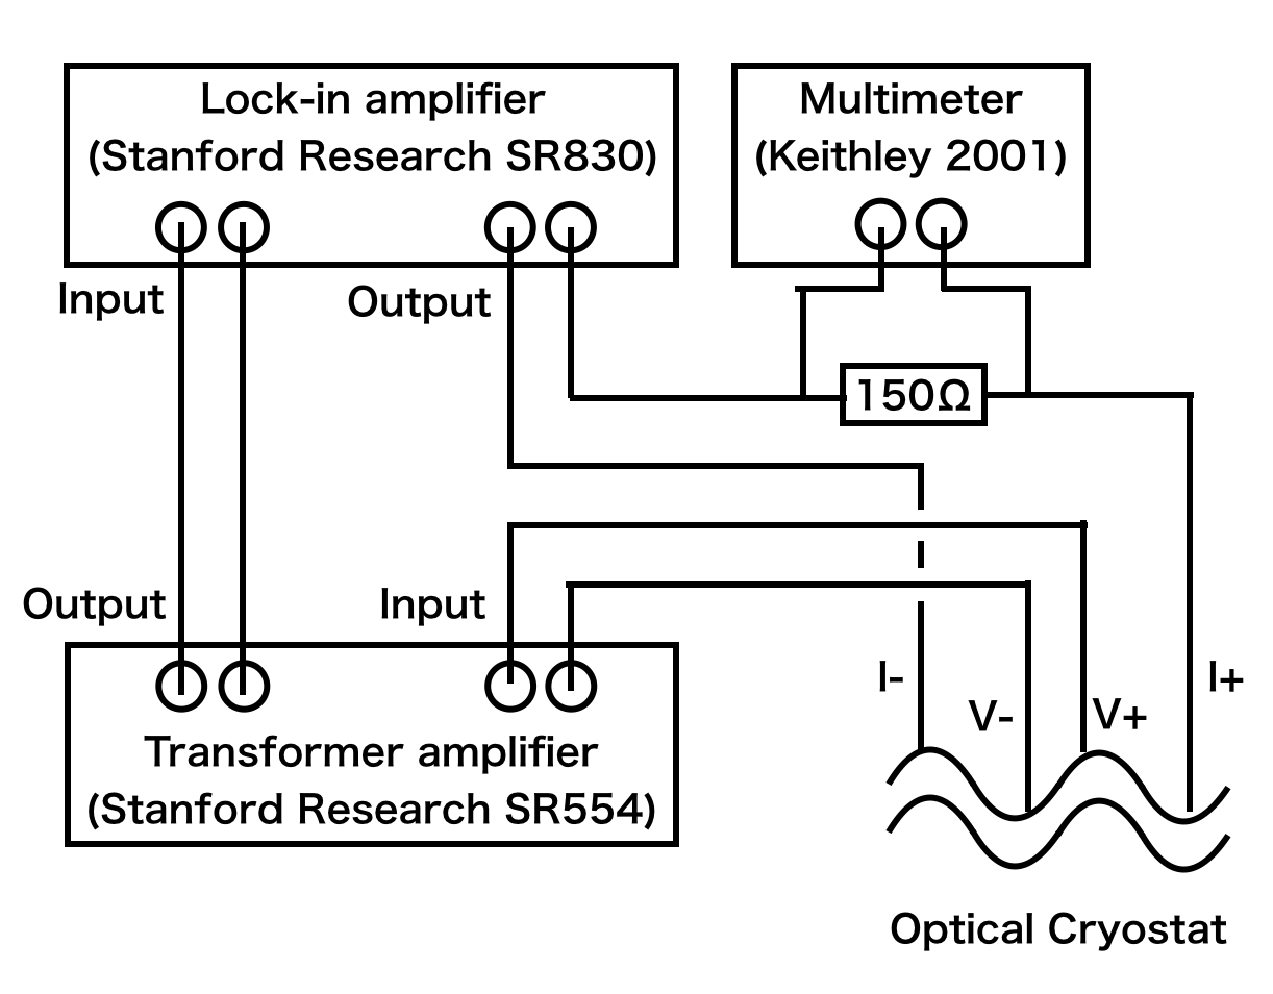
\includegraphics[width=\hsize]{experiment/schematics_pulse.eps}
  \end{center}
  \caption{}
  \label{fig:schematics_pulse}
 \end{minipage}
 \begin{minipage}{0.5\hsize}
     \begin{center}
   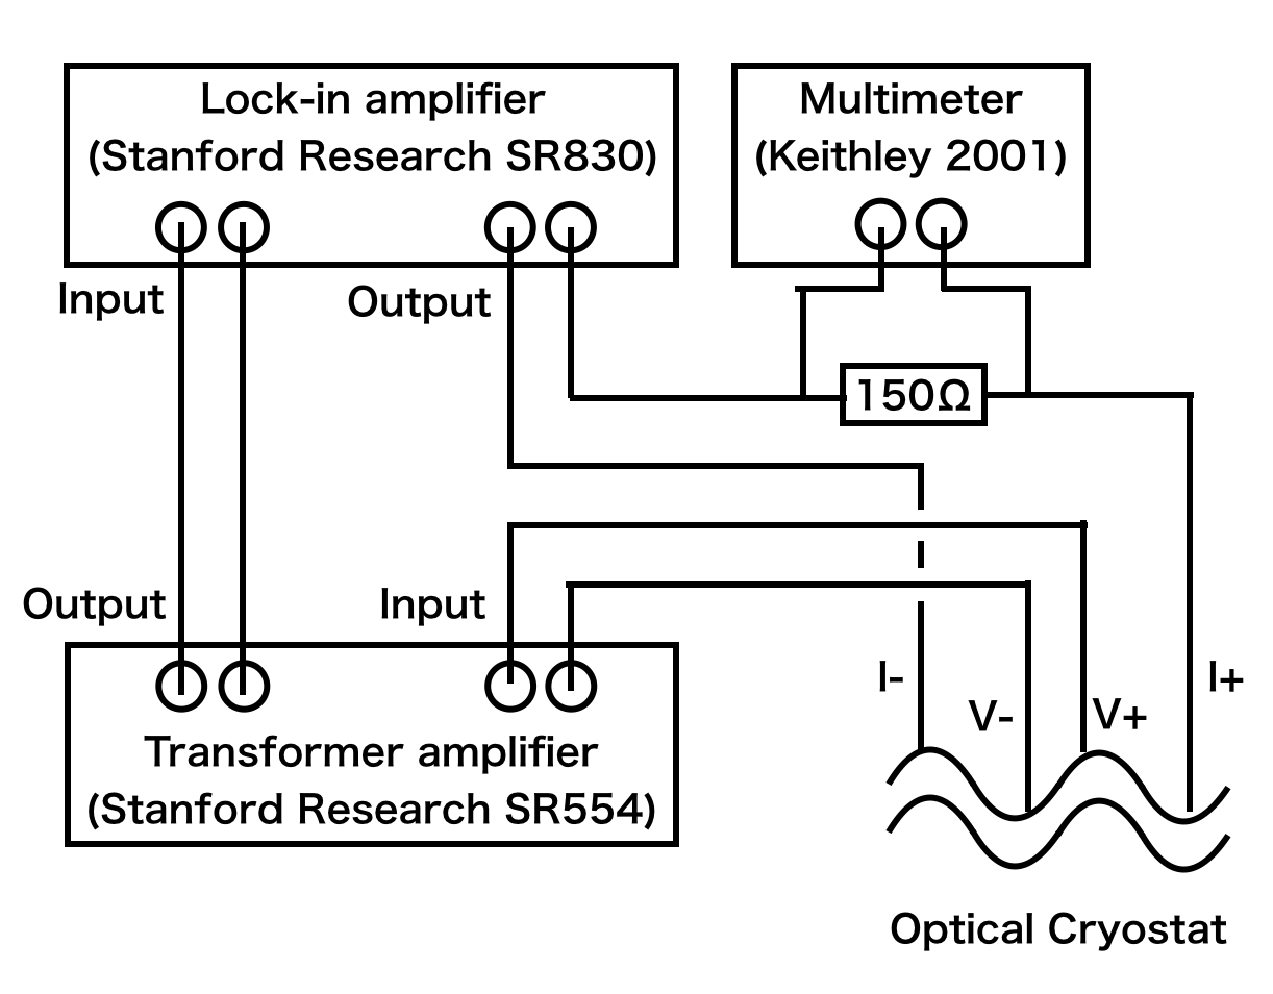
\includegraphics[width=\hsize]{experiment/schematics_lockin.eps}
  \end{center}
  \caption{}
  \label{fig:schematics_lockin}
   \end{minipage}
\end{figure}

\subsection{電流パルスによるα相とβ相の共存状態の生成}

\begin{figure}[htb]
 \begin{minipage}{0.4\hsize}
    \begin{center}
   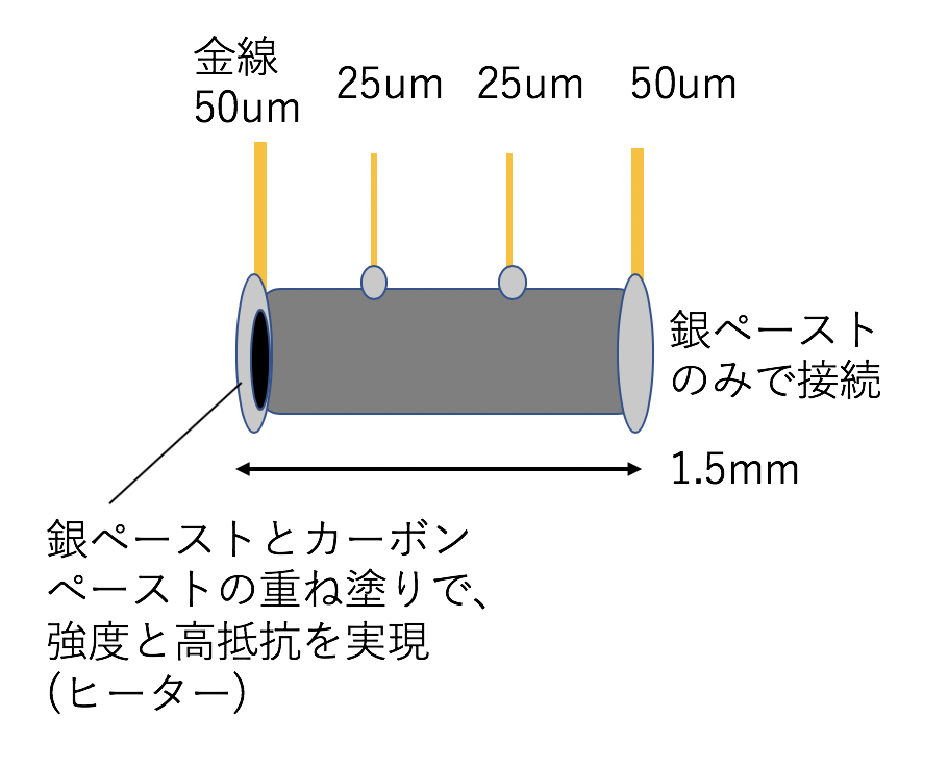
\includegraphics[width=\hsize]{experiment/schematics_sample.eps}
  \end{center}
  \caption{}
  \label{fig:schematics_sample}
 \end{minipage}
 \begin{minipage}{0.6\hsize}
     \begin{center}
   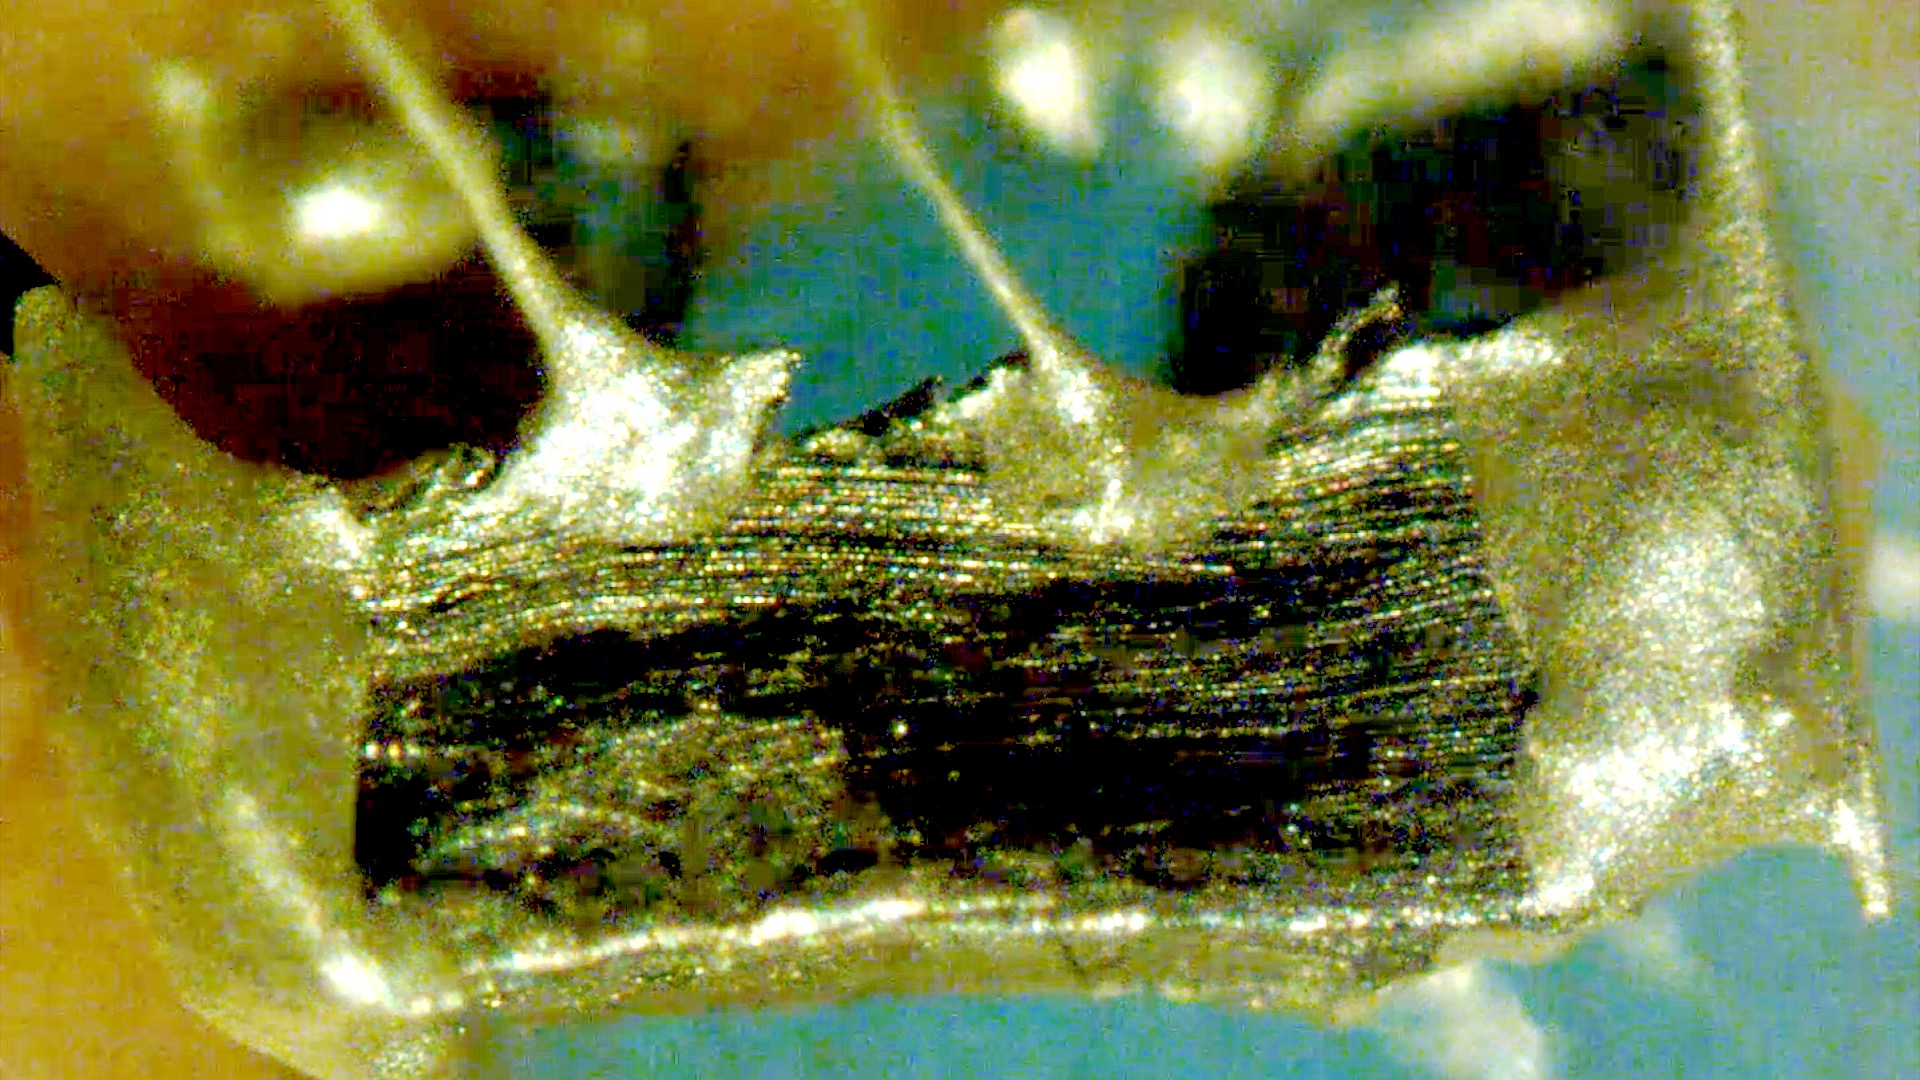
\includegraphics[width=\hsize]{experiment/picture_sample.eps}
  \end{center}
  \caption{}
  \label{fig:picture_sample}
   \end{minipage}
\end{figure}


α相とβ相の共存状態を観察するため、光学顕微鏡を構成した。

\subsection{電流パルスを用いたβ相からα相への変換}

\newpage

%\ref{sec:4terminal}